% Created with jtex v.0.1.15
\documentclass{article}
\usepackage{arxiv}

\usepackage[utf8]{inputenc} % allow utf-8 input
\usepackage[T1]{fontenc}    % use 8-bit T1 fonts
\usepackage{hyperref}       % hyperlinks
\usepackage{url}            % simple URL typesetting
\usepackage{datetime}       % show dates in the title block
\usepackage{booktabs}       % professional-quality tables
\usepackage{amsfonts}       % blackboard math symbols
\usepackage{nicefrac}       % compact symbols for 1/2, etc.
\usepackage{microtype}      % microtypography
\usepackage{graphicx}
\usepackage{natbib}
\usepackage{doi}
\usepackage{xcolor}

%%%%%%%%%%%%%%%%%%%%%%%%%%%%%%%%%%%%%%%%%%%%%%%%%%
%%%%%%%%%%%%%%%%%%%%  imports  %%%%%%%%%%%%%%%%%%%
\usepackage{amsmath}
%%%%%%%%%%%%%%%%%  math commands  %%%%%%%%%%%%%%%%
\newcommand{\DiscFac}{\beta}
\newcommand{\cFunc}{\mathrm{c}}
\newcommand{\uFunc}{\mathrm{u}}
\newcommand{\vFunc}{\mathrm{v}}
\newcommand{\Alive}{\mathcal{L}}
\newcommand{\h}{h}
\newcommand{\cLvl}{\mathbf{c}}
\newcommand{\mLvl}{\mathbf{m}}
\newcommand{\pLvl}{\mathbf{p}}
\newcommand{\Ex}{\mathbb{E}}
\newcommand{\CRRA}{\rho}
\newcommand{\PermGroFac}{\pmb{\Phi}}
\newcommand{\Rfree}{\mathsf{R}}
\newcommand{\PermShk}{\mathbf{\Psi}}
\newcommand{\TranShk}{\pmb{\xi}}
\newcommand{\aNrm}{a}
\newcommand{\cNrm}{c}
\newcommand{\RNrm}{\mathcal{R}}
\newcommand{\TranShkEmp}{\pmb{\theta}}
\newcommand{\mNrm}{m}
\newcommand{\pZero}{\wp}
\newcommand{\aFunc}{\mathrm{a}}
\newcommand{\kapShare}{\alpha}
\newcommand{\wealth}{o}
\newcommand{\kap}{k}
\newcommand{\wealthShare}{\delta}
\newcommand{\wFunc}{\mathrm{w}}
\newcommand{\aRat}{a}
\newcommand{\mRat}{m}
\newcommand{\aMat}{[\mathrm{a}]}
\newcommand{\mMat}{[\mathrm{m}]}
%%%%%%%%%%%%%%%%%%%%%%%%%%%%%%%%%%%%%%%%%%%%%%%%%%

\hypersetup{colorlinks = true,
linkcolor = purple,
urlcolor  = blue,
citecolor = cyan,
anchorcolor = black}

\title{Structural Estimation of Life Cycle Models with Wealth in the Utility Function}

\newdate{articleDate}{21}{6}{2023}
\date{\displaydate{articleDate}}

\makeatletter
\let\@fnsymbol\@arabic
\makeatother

\author{Alan Lujan\footnotemark[1]\\
Ohio State University\\Econ-ARK\\}

% Uncomment to override  the `A preprint' in the header
\renewcommand{\headeright}{Economics}
\renewcommand{\undertitle}{}
\renewcommand{\shorttitle}{Structural Estimation}

%% Add PDF metadata to help others organize their library
%% Once the PDF is generated, you can check the metadata with
%% $ pdfinfo template.pdf
\hypersetup{
pdftitle={\@title},
pdfsubject={},
pdfauthor={\@author},
pdfkeywords={structural estimation,life cycle,wealth in the utility},
addtopdfcreator={Written in Curvenote}
}

\begin{document}
\maketitle
\footnotetext[1]{Correspondence to: alanlujan91@gmail.com}

\begin{abstract}
Heterogeneous Agent Models (HAM) are a powerful tool for understanding the effects of monetary and fiscal policy on the economy. However, current state-of-the-art frameworks such as Heterogeneous Agent New Keynesian (HANK) models have limitations that hinder their ability to accurately replicate real-world economic phenomena. Specifically, HANK models struggle to account for the observed hoarding of wealth at the very top of the distribution and lack important life cycle properties such as time-varying mortality and income risk. On the one hand, the inability to pin down wealth at the tail of the distribution has been a problem for HANK models precisely because it has implications for the transmission of monetary and fiscal policy. On the other hand, agents in HANK are generally conceived as perpetual youth with infinite horizons and without age-specific profiles of mortality and income risk. This is problematic as it ignores the effects of these policies on potentially more affected communities, such as young families with children or the low-wealth elderly. In this paper, I investigate the effects of both life cycle considerations as well as wealth in the utility on the structural estimation of HAMs. Structural estimation is the first step in evaluating the effect of monetary and fiscal policies in a HANK framework, and my hope is that this paper will lead to better models of the economy that can be used to inform policy.
\end{abstract}

\keywords{structural estimation, life cycle, wealth in the utility}

%  Heterogeneous Agent Models (HAM) have become a popular tool for understanding the effects of monetary and fiscal policy on the economy. However, current state-of-the-art frameworks such as Heterogeneous Agent New Keynesian (HANK) models have limitations that hinder their ability to accurately replicate real-world economic phenomena. Specifically, HANK models struggle to account for the observed hoarding of wealth at the very top of the distribution and lack important life cycle properties such as time-varying mortality and income risk. These limitations are problematic because they affect the transmission of monetary and fiscal policy and ignore the effects of these policies on potentially more affected communities, such as young families with children or the low-wealth elderly.
% 
% To address these limitations, this paper investigates the effects of both life cycle considerations and wealth in the utility on the structural estimation of HAMs. By incorporating these factors into the model, we aim to provide a more accurate representation of the economy and its response to monetary and fiscal policy. Our research methodology involves using a combination of theoretical analysis and empirical data to estimate the parameters of the model.
% 
% Our findings suggest that incorporating life cycle considerations and wealth in the utility can significantly improve the accuracy of HAMs. This has important implications for policymakers who rely on these models to inform their decisions. By providing a more accurate representation of the economy, our research can help policymakers make better-informed decisions that benefit all members of society. Overall, we hope that our research will contribute to the development of better models of the economy that can be used to inform policy.

I would like to thank my advisor, Chris Carroll, for his guidance and support throughout this project. His expertise and mentorship have been invaluable in shaping my work. Additionally, I would like to extend my appreciation to the members of the \href{https://econ-ark.org/}{Econ-ARK} team for fostering a dynamic and collaborative community that has greatly enriched my experience. Their contributions and feedback have been instrumental in helping me achieve my goals. All remaining errors are my own. The figures in this paper were generated using the \href{https://github.com/econ-ark/HARK}{Econ-ARK/HARK} toolkit.

\section{Introduction}\label{Introduction}

\section{Life Cycle Incomplete Markets Models}\label{Life Cycle Incomplete Markets Models}

An important extension to the Standard Incomplete Markets (SIM) model is the Life Cycle Incomplete Markets (LCIM) model as in \cite{Cagetti_2003}, \cite{Gourinchas_2002}, and \cite{Palumbo_1999}, among others. The LCIM model is a natural extension to the SIM model that allows for age-specific profiles of preferences, mortality, and income risk.

\subsection{The Baseline Model}\label{The Baseline Model}

The agent's objective is to maximize present discounted utility from consumption over the life cycle with a terminal period of $T$:

\begin{equation}
\label{eq:lifecyclemax}
\vFunc_{t}(\pLvl_{t},\mLvl_{t})  =    \max_{\{\cFunc\}_{t}^{T}} ~ \uFunc(\cLvl_{t})+\Ex_{t}\left[\sum_{n=1}^{T-t} {\beth}^{n} \Alive_{t}^{t+n}\hat{\DiscFac}_{t}^{t+n} \uFunc(\cLvl_{t+n}) \right]
\end{equation}

where $\pLvl_{t}$ is the permanent income level, $\mLvl_{t}$ is total market resources, $\cLvl_{t}$ is consumption, and

\begin{equation}
\begin{align}
    \beth & :  \text{time-invariant `pure' discount factor}
    \\ \Alive _{t}^{t+n} & :  \text{probability to }\Alive\text{ive until age $t+n$ given alive at age $t$}
    \\ \hat{\DiscFac}_{t}^{t+n} & :  \text{age-varying discount factor between ages $t$ and $t+n$.}
\end{align}
\end{equation}

It will be convenient to work with the problem in permanent-income-normalized form as in \cite{Carroll_2004}, which allows us to reduce a 2 dimensional problem of permanent income and wealth into a 1 dimensional problem of wealth normalized by permanent income. The recursive Bellman equation can be expressed as:

\begin{equation}
\begin{align}
    {\vFunc}_{t}({m}_{t}) & = \max_{\cNrm_{t}} ~ \uFunc(\cNrm_{t})+\beth\Alive_{t+1}\hat{\DiscFac}_{t+1}
    \Ex_{t}[(\PermShk_{t+1}\PermGroFac_{t+1})^{1-\CRRA}{\vFunc}_{t+1}({m}_{t+1})]
    \\ & \text{s.t.} & 
    \\ \aNrm_{t} & = {m}_{t}-\cNrm_{t} 
    \\ {m}_{t+1} & = \aNrm_{t}\underbrace{\left(\frac{\Rfree}{\PermShk_{t+1}\PermGroFac_{t+1}}\right)}_{\equiv \RNrm_{t+1}}
    + ~\TranShkEmp_{t+1}
\end{align}
\end{equation}

where $\cNrm$, $\aNrm$, and $\mNrm$ are consumption, assets, and market resources normalized by permanent income, respectively, $\vFunc$ and $\uFunc$ are now the normalized value and utility functions,  and

\begin{equation}
\begin{align}
  \PermShk_{t+1} & :  \text{mean-one shock to permanent income}
    \\ \PermGroFac_{t+1} & :  \text{permanent income growth factor}
    \\ \TranShkEmp_{t+1} & :  \text{transitory shock to permanent income}
    \\ \RNrm_{t+1} & :  \text{permanent income growth normalized return factor}
\end{align}
\end{equation}

with all other variables are defined as above. The transitory and permanent shocks to income are defined as:

\begin{equation}
\begin{align}
\TranShkEmp_{s}  = &
    \begin{cases}
        0\phantom{/\pZero} & \text{with probability $\pZero>0$}
        \\ \xi_{s}/\pZero & \text{with probability $(1-\pZero)$, where
            $\log \xi_{s}\thicksim \mathcal{N}(-\sigma_{[\xi, t]}^{2}/2,\sigma_{[\xi, t]}^{2})$}
    \end{cases}
    \\ \phantom{/\pZero} \\ & \text{and }  \log \PermShk_{s}   \thicksim \mathcal{N}(-\sigma_{[\PermShk, t]}^{2}/2,\sigma_{[\PermShk, t]}^{2}).
  \end{align}
\end{equation}

\subsection{Wealth in the Utility Function}\label{Wealth in the Utility Function}

A simple extension to the Life Cycle Incomplete Markets (LCIM) model is to include wealth in the utility function. \cite{Carroll_1998} argues that models in which the only driver of wealth accumulation is consumption smoothing are not consistent with the saving behavior of the wealthiest households. Instead, they propose a model in which households derive utility from their level of wealth itself or they derive a flow of services from political power and social status, calling it the `Capitalist Spirit' model. In turn, we can add this feature to the LCIM model by adding a utility function with consumption and wealth as follows:

\begin{equation}
\begin{align}
    {\vFunc}_{t}({m}_{t}) & = \max_{\cNrm_{t}} ~ \uFunc(\cNrm_{t}, \aNrm_{t})+\beth\Alive_{t+1}\hat{\DiscFac}_{t+1}
    \Ex_{t}[(\PermShk_{t+1}\PermGroFac_{t+1})^{1-\CRRA}{\vFunc}_{t+1}({m}_{t+1})]
    \\ & \text{s.t.} & 
    \\ \aNrm_{t} & = {m}_{t}-\cNrm_{t} 
    \\ {m}_{t+1} & = \aNrm_{t}\RNrm_{t+1}+ ~\TranShkEmp_{t+1}
\end{align}
\end{equation}

\textbf{Separable Utility} \cite{Carroll_1998} presents extensive empirical and informal evidence for a LCIM model with wealth in the utility function. Specifically, the paper uses a utility that is separable in consumption and wealth:

\begin{equation}
\uFunc(\cNrm_{t}, \aNrm_{t}) = \frac{\cNrm_{t}^{1-\CRRA}}{1-\CRRA}
    + \kapShare_{t} \frac{(\aFunc_{t} - \underline\aNrm)^{1-\wealthShare}}{1-\wealthShare}
\end{equation}

where $\kapShare$ is the relative weight of the utility of wealth and $\wealthShare$ is the relative risk aversion of wealth.

\textbf{Non-separable Utility} A different model that we will explore is one in which the utility function is non-separable in consumption and wealth; i.e. consumption and wealth are complimentary goods. In the case of the LCIM model, this dynamic complementarity drives the accumulation of wealth not only for the sake of wealth itself, but also because it increases the marginal utility of consumption.

\begin{equation}
\uFunc(\cNrm_{t}, \aNrm_{t}) = \frac{(\cNrm_{t}^{1-\wealthShare} (\aNrm_{t} - \underline\aNrm)^\wealthShare)^{1-\CRRA}}{(1-\CRRA)}
\end{equation}

\section{Solution Methods}\label{Solution Methods}

For a brief departure, let's consider how we solve these problems generally. Define the post-decision value function as:

\begin{equation}
\begin{align}
    \DiscFac_{t+1} \wFunc_{t}(\aNrm_{t}) & = \beth\Alive_{t+1}\hat{\DiscFac}_{t+1}
    \Ex_{t}[(\PermShk_{t+1}\PermGroFac_{t+1})^{1-\CRRA}{\vFunc}_{t+1}({m}_{t+1})]
    \\ & \text{s.t.}
    \\ {m}_{t+1} & = \aNrm_{t}\RNrm_{t+1}+ ~\TranShkEmp_{t+1}
\end{align}
\end{equation}

For our purposes, it will be useful to simplify the notation a bit by dropping time subscripts. The recursive problem can then be written as:

\begin{equation}
\begin{align}
    \vFunc(\mRat) & = \max_{\cNrm} ~ \uFunc(\cNrm, \aNrm) + \DiscFac \wFunc(\aRat)
    \\ & \text{s.t.}
    \\ \aNrm & = \mRat-\cNrm
\end{align}
\end{equation}

\subsection{Endogenous Grid Method, Abridged}\label{Endogenous Grid Method, Abridged}

In the standard incomplete markets (SIM) model, the utility function is simply $\uFunc(\cNrm)$ and the Euler equation is $\uFunc'(\cNrm) = \DiscFac \wFunc'(\aNrm)$, which is a necessary and sufficient condition for an internal solution of the optimal choice of consumption. If $\uFunc(\cNrm)$ is differentiable and its marginal utility is invertible, then the Euler equation can be inverted to obtain the optimal consumption function as $\cNrm(\aNrm) = \uFunc'^{ -1}(\DiscFac \wFunc'(\aNrm))$. Using an \textit{exogenous} grid of post-decision savings $\aMat$, we can obtain an \textit{endogenous} grid of market resources $\mMat$ by using the budget constraint $\mNrm(\aMat) = \aMat + \cNrm(\aMat)$ such that this collection of grids satisfy the Euler equation. This is the endogenous grid method (EGM) of \cite{Carroll_2006}.

In the presence of wealth in the utility function, the Euler equation is more complicated and may not be invertible in terms of optimal consumption. Consider the first order condition for an optimal combination of consumption and savings, denoted by $^*$:

\begin{equation}
\uFunc_{c}'(\cNrm^*, \aNrm^*) - \uFunc_{a}'(\cNrm^*, \aNrm^*) = \DiscFac \wFunc'(\aNrm^*)
\end{equation}

If the utility of consumption and wealth is additively separable, then the Euler equation can be written as $\uFunc_{c}'(\cNrm) = \uFunc_{a}'(\aNrm) + \DiscFac \wFunc'(\aNrm)$. This makes sense, as the agent will equalize the marginal utility of consumption with the marginal utility of wealth today plus the discounted marginal value of wealth tomorrow. In this case, the EGM is simple: we can invert the Euler equation to obtain the optimal consumption policy as $\cNrm(\aNrm) = \uFunc_{c}'^{ -1}\big(\uFunc_{a}'(\aNrm) + \DiscFac \wFunc'(\aNrm)\big)$. We can proceed with EGM as usual, using the budget constraint to obtain the endogenous grid of market resources $\mNrm(\aMat) = \aMat + \cNrm(\aMat)$.

\section{Quantitative Strategy}\label{Quantitative Strategy}

This section describes the quantitative strategy used for calibrating and estimating the Life Cycle Incomplete Markets model with and without Wealth in the Utility Function, following the works of \cite{Cagetti_2003}, \cite{Palumbo_1999}, \cite{Gourinchas_2002}, and \cite{Sabelhaus_2010}, among others. The main objective is to find a set of parameters that can best match the empirical moments of some real-life data using simulation.

\subsection{Calibration}\label{Calibration}

The calibration of the Life Cycle Incomplete Markets model necessitates a richness not present in the SIM model precisely because we are interested in the heterogeneity of agents across different stages of the life cycle, such as the early working period, parenthood, saving for retirement, and retirement. To calibrate this model, we need to identify important patterns in preferences, mortality, and income risk across the life cycle. The first and perhaps most important departure from SIM is that life is finite and agents don't life forever; moreover, the terminal age is not certain as the probability of staying alive decreases with age. In this model, households start their life cycle at age $t = 25$ and live with certainty until retirement at age $t = 65$. After retirement, the probability of staying alive decreases with age, and the terminal age is set to $t = 91$. During their early adulthood, their utility of consumption might need to be adjusted by the arrival and subsequent departure of children. This is handled by a `household-size-adjusted' discount factor that is greater than 1.0 in the presence of children. This is the rationale for parameters $\Alive_{t}$ and $\hat{\DiscFac}_{t}$ in the model, whose values we take from \cite{Cagetti_2003} directly.

The unemployment probability is taken from \cite{Carroll_1992} to be $\pZero = 0.5$ which represents a long run equilibrium of 5\% unemployment in the United States. The remaining life cycle attributes for the distribution of shocks to income ($\PermGroFac_{t}, \ \sigma_{[\PermShk, t]}, \ \sigma_{[\xi, t]}$) are taken from \cite{Sabelhaus_2010}. In their paper, they analyze the variability of labor earnings growth rates between the 80's and 90's and find evidence for the "Great Moderation", a decline in variability of earnings across all age groups.

After careful calibration based on the Life Cycle Incomplete Markets literature, we can structurally estimate the remaining parameters $\beth$ and $\CRRA$ to match specific empirical moments of the wealth distribution.

\subsection{Estimation}\label{Estimation}

\begin{figure}[!htbp]
\centering
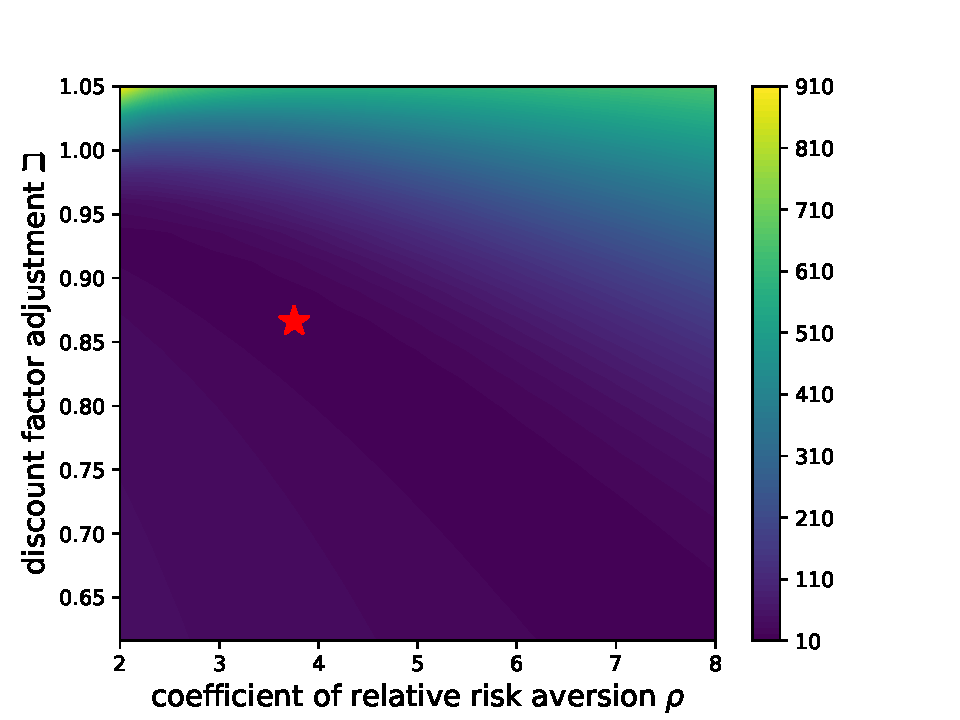
\includegraphics[width=0.7\linewidth]{files/IndShockSMMcontour-f950f8faf8926e47605d36d01964a2f6.pdf}
\caption{Contour plot of the objective function for the structural estimation of the Life Cycle Incomplete Markets model. The red dot represents the estimated parameters.}
\label{fig:IndShockSMMcontour}
\end{figure}

\begin{figure}[!htbp]
\centering
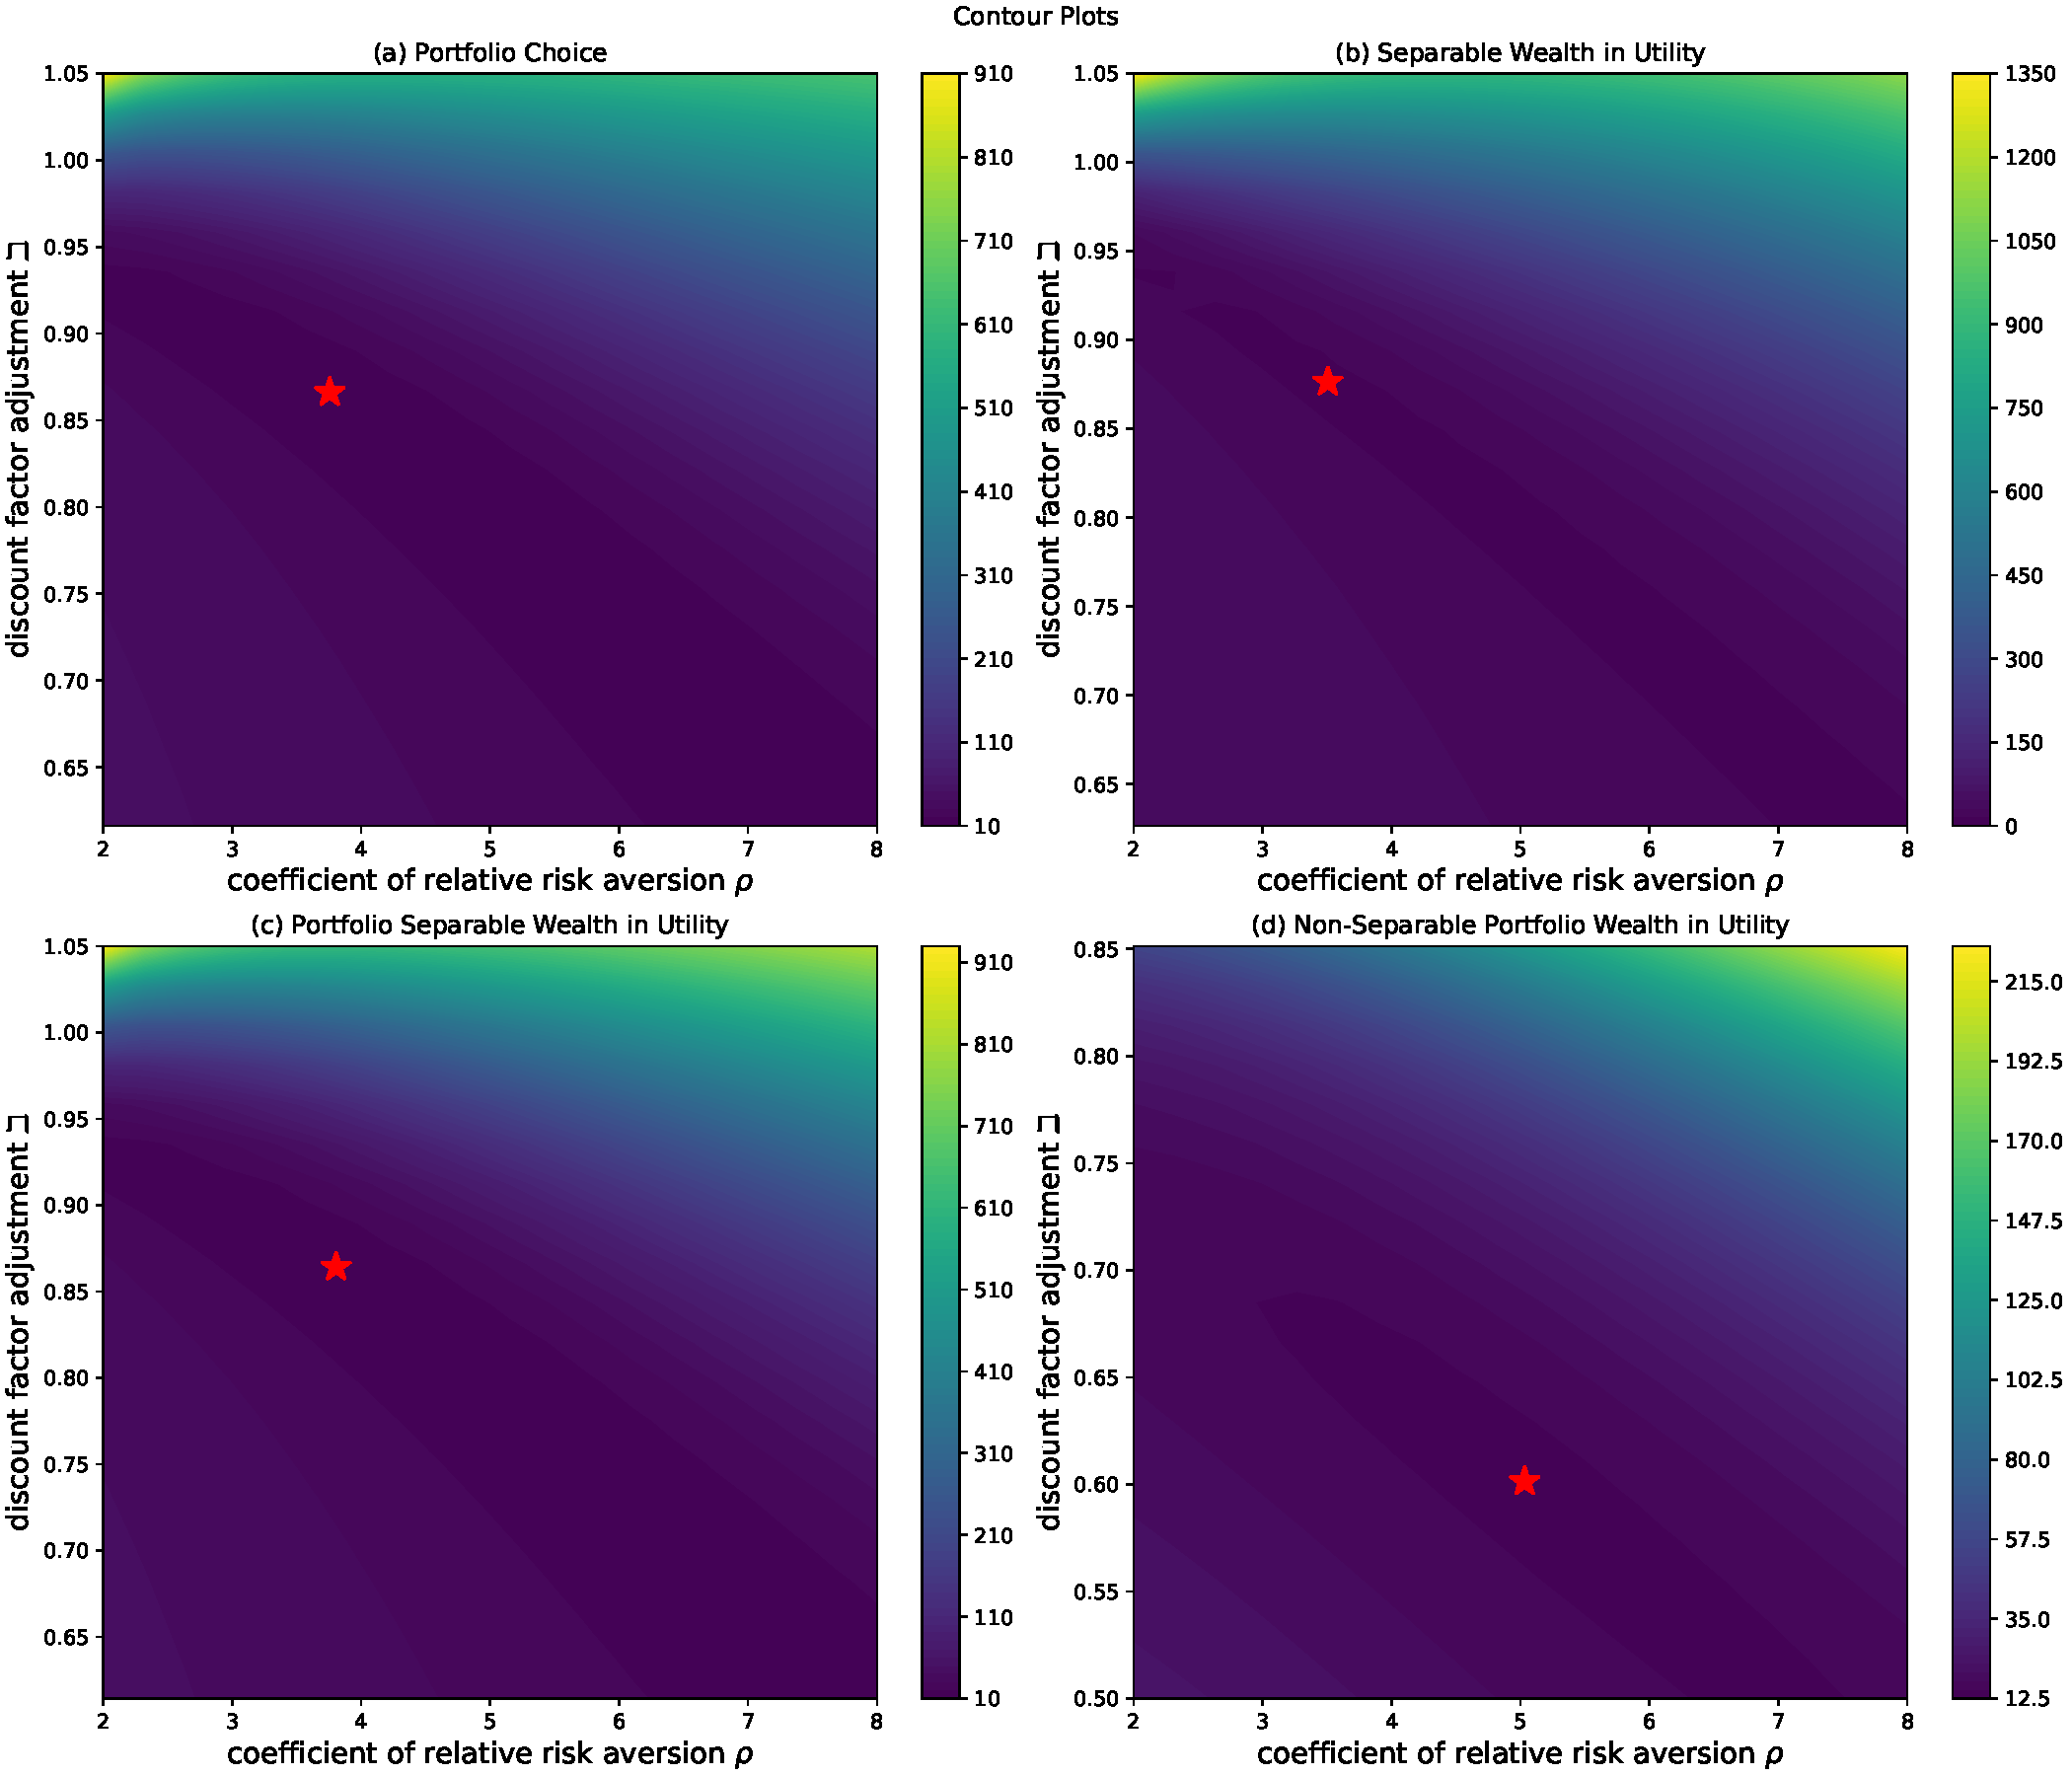
\includegraphics[width=0.7\linewidth]{files/AllSMMcontour-61083533183861c53042688308f7803e.pdf}
\caption{Contour plot of the objective function for the structural estimation of the Life Cycle Incomplete Markets model. The red dot represents the estimated parameters.}
\label{fig:AllSMMcontour}
\end{figure}

\subsection{Sensitivity Analysis}\label{Sensitivity Analysis}

For our sensitivity analysis, we use the methods introduced by \cite{Andrews_2017}.

\begin{figure}[!htbp]
\centering
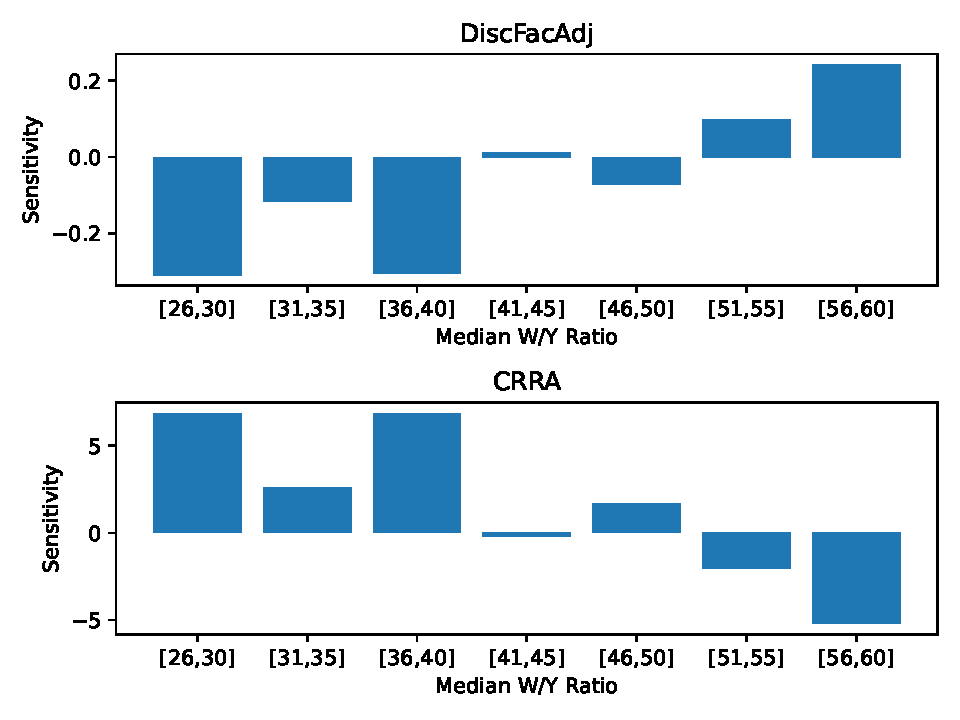
\includegraphics[width=0.7\linewidth]{files/IndShockSensitivity-9046783d8c17a2fc3e39f5fb5ebcf6c7.pdf}
\caption{Sensitivity analysis of the structural estimation of the Life Cycle Incomplete Markets model. The red dot represents the estimated parameters.}
\label{fig:IndShockSensitivity}
\end{figure}

\begin{figure}[!htbp]
\centering
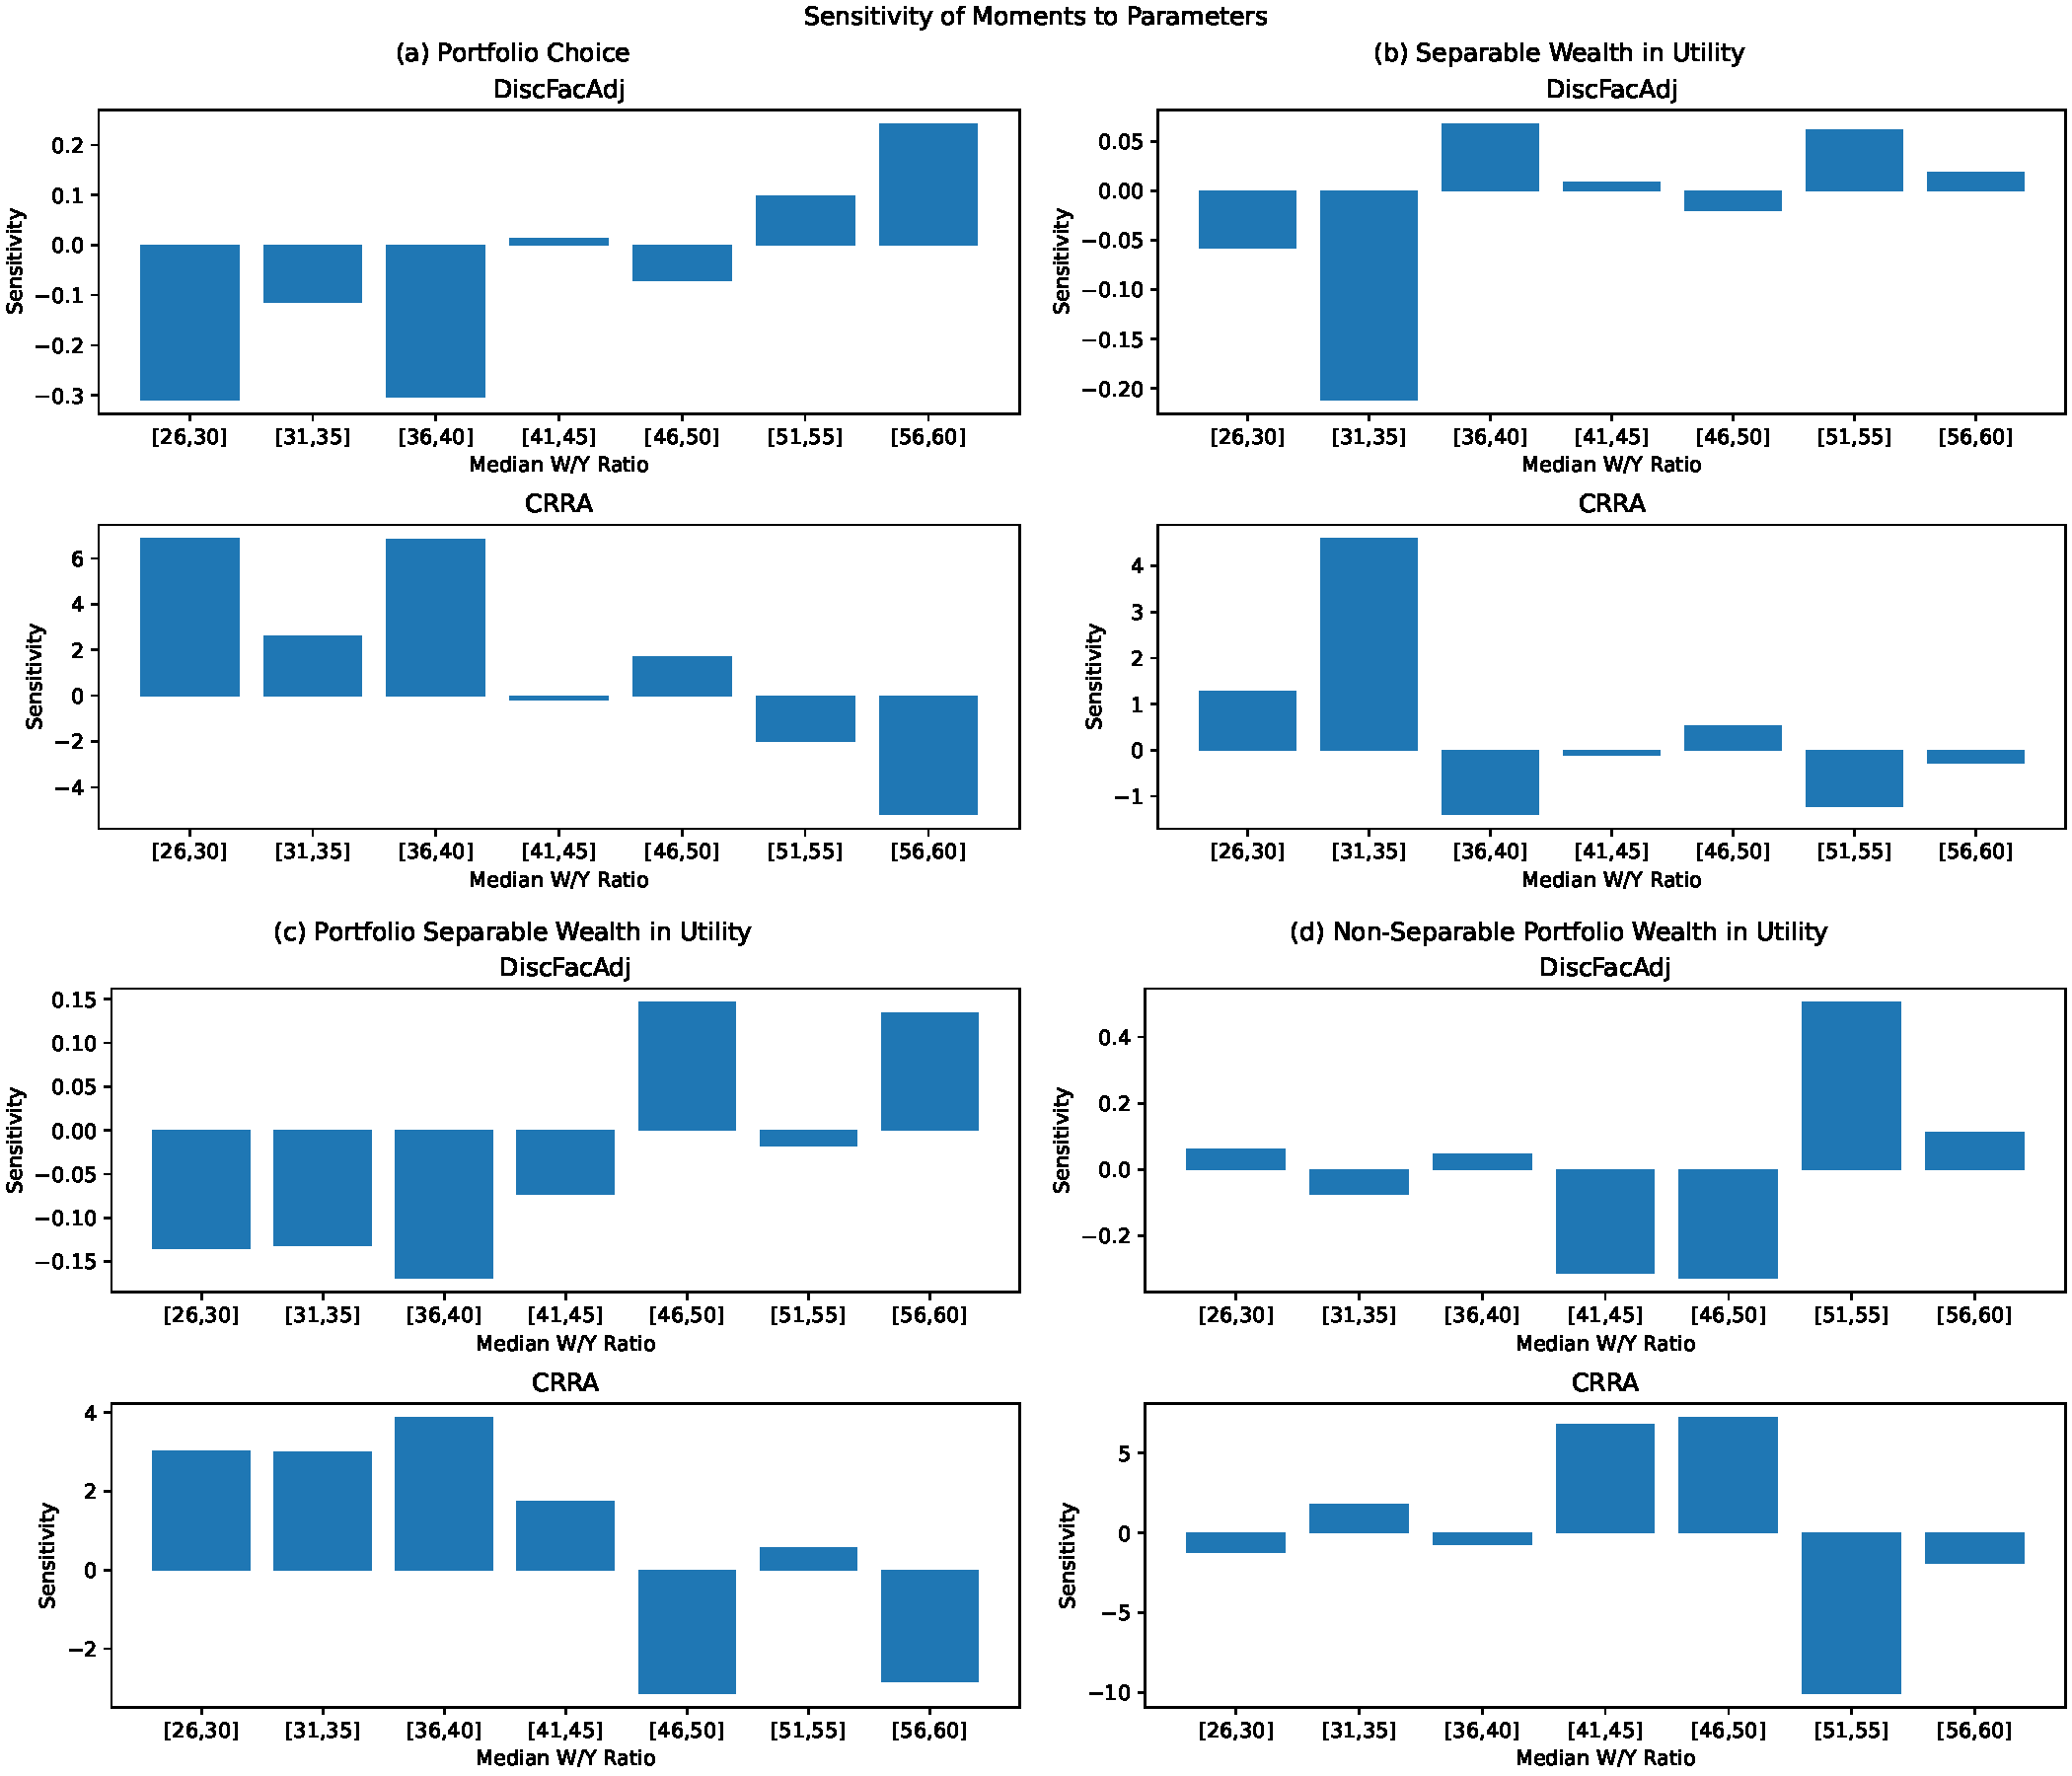
\includegraphics[width=0.7\linewidth]{files/AllSensitivity-0f14236654de527c752f26a13f644a4c.pdf}
\caption{Sensitivity analysis of the structural estimation of the Life Cycle Incomplete Markets model. The red dot represents the estimated parameters.}
\label{fig:AllSensitivity}
\end{figure}

\section{Conclusion}\label{Conclusion}

\section{References}\label{References}

\cite{Palumbo_1999}
\cite{Carroll_2000}
\cite{Carroll_1998}
\cite{Michaillat_2021}
\cite{Auclert_2021}
\cite{Mian_2020}
\cite{Kaplan_2018}
\cite{Auclert_2020}
\cite{Cagetti_2003}
\cite{Andrews_2017}
\cite{Attanasio_1999}  
%  Humps and Bumps in Lifetime Consumption



\bibliographystyle{unsrtnat}
\bibliography{main.bib}

\end{document}
